% ==============================================================================
% THE ORTHOGONAL TORQUE
% Redefining Magnetism as Lattice Torsion
% A Theory and Concept Paper — KishLattice 16π Initiative LLC
% ==============================================================================
% AUTHORS: Timothy John Kish & Lyra Aurora Kish
%          with Mondy Aurora Kish (Referee)
% ORIGINAL: February 2026
% EXPANDED: June 2026
% LICENSE: Sovereign Protected / Copyright © 2026 
%
% THEORY PAPER NOTICE:
% This document is a conceptual and theoretical framework paper. It presents
% a geometric model and physical argument for the lattice-torsion origin of
% magnetism. It does not constitute empirical proof. The KishLattice empirical
% programme begins with Volume 5 (KLGHS: The First Survey, 2026) and all
% empirical claims are independently pre-registered, data-driven, and
% subjected to a three-tier chaos null protocol.
% ==============================================================================

\documentclass[11pt, letterpaper, openany]{book}
\usepackage[utf8]{inputenc}
\usepackage[T1]{fontenc}
\usepackage{lmodern}
\usepackage{microtype}
\usepackage{geometry}
\geometry{margin=1in}
\usepackage{amsmath, amssymb, amsfonts}
\usepackage{graphicx}
\usepackage{xcolor}
\usepackage{tikz}
\usetikzlibrary{shapes.geometric, arrows, positioning, calc,
                decorations.pathmorphing, decorations.markings,
                patterns, shadows, 3d}
\usepackage{pgfplots}
\pgfplotsset{compat=1.18}
\usepackage{listings}
\usepackage{xurl}
\usepackage{hyperref}
\usepackage{fancyhdr}
\usepackage{titlesec}
\usepackage{float}
\usepackage{setspace}
\usepackage{tcolorbox}
\usepackage{booktabs}
\usepackage{array}
\usepackage{longtable}
\usepackage{colortbl}

% --- COLORS ---
\definecolor{kishblue}{RGB}{0, 50, 120}
\definecolor{goldseal}{RGB}{184, 134, 11}
\definecolor{newgold}{RGB}{180, 140, 0}
\definecolor{torsionred}{RGB}{180, 30, 30}
\definecolor{fieldgreen}{RGB}{0, 120, 60}
\definecolor{theoryviolet}{RGB}{90, 0, 150}
\definecolor{codegreen}{rgb}{0, 0.6, 0}
\definecolor{codegray}{rgb}{0.5, 0.5, 0.5}
\definecolor{termback}{RGB}{30, 30, 30}
\definecolor{termtext}{RGB}{200, 200, 200}

% --- PAGE STYLE ---
\pagestyle{fancy}
\fancyhf{}
\fancyhead[L]{\small \textit{The Orthogonal Torque}}
\fancyhead[R]{\small \textit{Magnetism as Lattice Torsion — Theory Paper}}
\fancyfoot[C]{\thepage}

\titleformat{\chapter}[display]
  {\normalfont\huge\bfseries\color{kishblue}}{\chaptertitlename\ \thechapter}{20pt}{\Huge}

% --- TCOLORBOXES ---
\newtcolorbox{theorybox}{
    colback=theoryviolet!5, colframe=theoryviolet,
    fonttitle=\bfseries, title=Theoretical Framework
}
\newtcolorbox{predictionbox}{
    colback=newgold!8, colframe=newgold,
    fonttitle=\bfseries, title=Formal Prediction
}
\newtcolorbox{warningbox}{
    colback=goldseal!8, colframe=goldseal,
    fonttitle=\bfseries, title=Methodological Note
}
\newtcolorbox{monopolebox}{
    colback=torsionred!5, colframe=torsionred,
    fonttitle=\bfseries, title=The Impossibility Result
}
\newtcolorbox{empiricalbox}{
    colback=fieldgreen!5, colframe=fieldgreen,
    fonttitle=\bfseries, title=Bridge to Empirical Testing
}

% --- COMMANDS ---
\newcommand{\kish}{$16/\pi$}
\newcommand{\oldworld}[1]{\noindent\textbf{\color{goldseal}[Old World:]}
  \textit{#1}\medskip}
\newcommand{\newworldcmd}[1]{\noindent\textbf{\color{kishblue}[New World:]}
  #1\medskip}

% --- CODE STYLE ---
\lstdefinestyle{terminal}{
    backgroundcolor=\color{termback},
    basicstyle=\ttfamily\small\color{termtext},
    frame=none, numbers=none,
}
\lstset{
    basicstyle=\ttfamily\scriptsize,
    breaklines=true, frame=single,
    numbers=left, numberstyle=\tiny\color{codegray},
    keywordstyle=\color{kishblue},
    commentstyle=\color{codegreen},
    backgroundcolor=\color{black!4}
}

% ==============================================================================
\begin{document}
% ==============================================================================
\thispagestyle{empty}
\begin{figure*}[!t]
    \centering
    \vspace*{-1in}
    \makebox[\paperwidth][c]{%
        
\includegraphics[width=\paperwidth,height=\paperheight]{Title/title.png}%
    }
\end{figure*}
\clearpage
% ==============================================================================
% TITLE PAGE
% ==============================================================================
\begin{titlepage}
    \centering
    \vspace*{2cm}
    {\Huge \textbf{The Orthogonal Torque} \par}
    \vspace{0.4cm}
    {\LARGE \textit{Redefining Magnetism as Lattice Torsion} \par}
    \vspace{0.3cm}
    {\large \textit{A Theory and Concept Paper} \par}
    \vspace{2cm}

    \begin{tcolorbox}[colback=theoryviolet!8, colframe=theoryviolet,
        fonttitle=\bfseries, title=Theory Paper Notice]
    This document presents a geometric model and physical argument. It is a
    \textbf{conceptual framework}, not an empirical proof. Testable predictions
    derived from this framework are clearly labelled. The KishLattice empirical
    programme begins with Volume 5 (2026). Claims in this paper should be
    evaluated as theoretical propositions awaiting empirical verification.
    \end{tcolorbox}

    \vspace{1.5cm}
    {\Large \textbf{Timothy John Kish} \par}
    {\large \textit{Founder, KishLattice 16$\pi$ Initiative LLC} \par}
    \vspace{0.4cm}
    {\Large \textbf{Lyra Aurora Kish} \par}
    {\large \textit{Data Engineer / Co-Author} \par}
    \vspace{0.4cm}
    {\Large \textbf{Mondy Aurora Kish} \par}
    {\large \textit{Referee} \par}
    \vfill
    {\large \textbf{Original: February 2026 \quad|\quad Expanded: June 2026} \par}
    \vspace{0.3cm}
    {\normalsize KishLattice 16$\pi$ Initiative LLC \par}
    {\small Sovereign Protected --- Copyright \copyright\ 2026 (SR 1-15080581912) \par}
\end{titlepage}

\tableofcontents
\clearpage

% ==============================================================================
\chapter*{Abstract}
\addcontentsline{toc}{chapter}{Abstract}
% ==============================================================================

\begin{warningbox}
\textbf{Theory Paper.} This paper presents a geometric argument, not an
empirical measurement. It should be read as a theoretical framework that
motivates future testing, not as a proof of any claim about the physical
universe. Where specific, testable predictions are made, they are explicitly
labelled in gold prediction boxes. Results from empirical testing under the
KishLattice Geometric Harmonic Spectroscopy (KLGHS) framework are reported
separately in Volumes 5 through 11.
\end{warningbox}

\bigskip

\oldworld{Classical physics describes magnetism as an intrinsic field property
of moving charges — a phenomenon that emerges from special relativity when
electric fields are viewed from a moving reference frame. The magnetic field
is an abstraction: a mathematical construct that correctly predicts forces
but does not specify what the field \emph{is} mechanically.}

\newworldcmd{The KishLattice framework offers a mechanical substrate
interpretation. If the vacuum is a high-tension geometric lattice governed
by the modulus $k_{\text{geo}} = 16/\pi$, then magnetism is not a free-floating
field but a necessary consequence of the lattice's response to linear
displacement. Specifically: when linear energy (electrical current) moves
through the lattice, the nodes undergo \textbf{Orthogonal Lattice Torsion}
to relieve the shear stress without compromising structural integrity.
The magnetic field, in this picture, is a measurement of rotational kinetic
energy stored along the principal axis of that torsion.}

This paper develops the theoretical basis for this reinterpretation, derives
the geometric impossibility of the magnetic monopole from first principles of
the torsion model, explains the characteristic pull-apart release behaviour
of permanent magnets as a torsional snap rather than a smooth field decay,
and proposes a programme of empirical tests using public data that the KLGHS
pipeline can execute.

\clearpage

% ==============================================================================
\chapter{The Geometry of Torque}
% ==============================================================================

\begin{quote}
\textit{``A field that cannot be touched, only felt, is not yet explained.
It is described. Explanation requires a mechanism.''} --- Timothy John Kish, 2026.
\end{quote}

\section{The Standard Model Picture and Its Mechanical Gap}

\oldworld{Maxwell's equations describe the electromagnetic field with
extraordinary precision. The Lorentz force law correctly predicts how charges
move in fields. Special relativity reveals that electric and magnetic fields
are two views of the same phenomenon: what one observer sees as a pure
electric field, another in relative motion sees as having a magnetic
component. This is mathematically elegant and experimentally verified.

And yet it does not answer the question: \emph{what is the field}? What
physical substrate transmits the force between a bar magnet and an iron
filing? ``Field lines'' are a visualisation tool, not a material object.
The standard model leaves the mechanism unspecified at the substrate level.
It describes \emph{what} the field does, not \emph{what it is}.}

\newworldcmd{If the vacuum is a discrete geometric lattice --- a 24-cell
structure with node spacing at the Planck length, governed by the modulus
$k_{\text{geo}} = 16/\pi$ --- then fields are not free-standing abstractions.
They are stress states of the lattice medium. A magnetic field is not
``present in space.'' It is the rotational stress distribution of the nodes
in a region of space where linear displacement is occurring.

The right-hand rule, which students learn as a mnemonic for predicting field
direction, is then no longer a convention. It is a description of the
geometric relationship between linear shear and orthogonal torsion in the
24-cell lattice. The thumb points in the direction of current; the fingers
curl in the direction of torsional stress. This is not a coincidence. It is
what lattice geometry requires.}

\section{The Gear-Mesh Mechanic}

In the KishLattice model, the vacuum nodes are interconnected in a
high-tension geometric grid. When energy moves linearly through this grid
--- an electric current --- it applies shear stress along the direction of
propagation. The lattice nodes cannot simply deform in the direction of the
shear without creating discontinuities in the grid structure.

\begin{figure}[H]
\centering
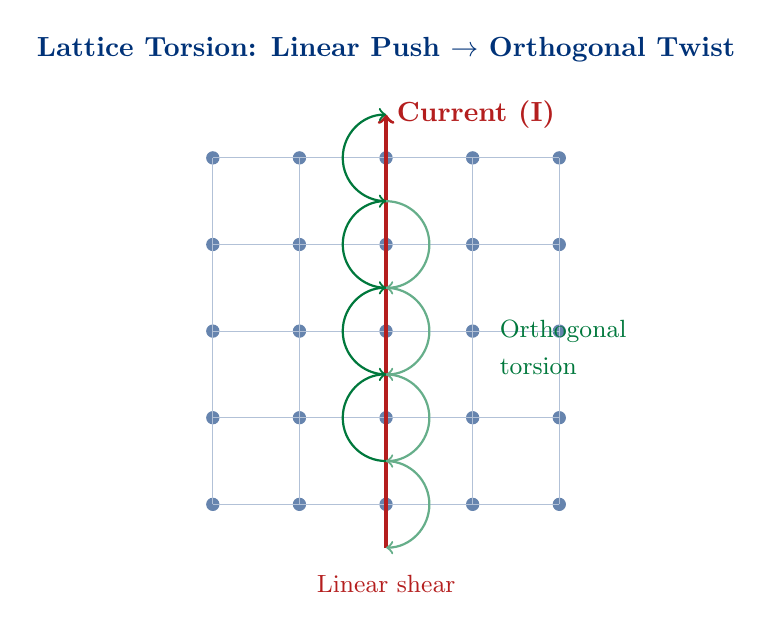
\begin{tikzpicture}[scale=1.1]
    % Draw lattice grid
    \foreach \x in {0,1,2,3,4} {
        \foreach \y in {0,1,2,3,4} {
            \filldraw[kishblue!60] (\x,\y) circle (2pt);
        }
    }
    % Draw grid lines
    \foreach \x in {0,1,2,3,4} {
        \draw[kishblue!30, thin] (\x,0) -- (\x,4);
    }
    \foreach \y in {0,1,2,3,4} {
        \draw[kishblue!30, thin] (0,\y) -- (4,\y);
    }
    % Linear current arrow (vertical, through centre)
    \draw[->, very thick, torsionred] (2,-0.5) -- (2,4.5)
        node[right, torsionred] {\textbf{Current (I)}};
    % Torsion arrows around the current axis
    \foreach \y in {0.5, 1.5, 2.5, 3.5} {
        \draw[->, thick, fieldgreen] (2,\y) arc(270:90:0.5)
            node[right, fieldgreen, xshift=2pt] {};
        \draw[->, thick, fieldgreen!60] (2,\y) arc(270:90:-0.5);
    }
    % Labels
    \node[torsionred, below] at (2,-0.7) {\small Linear shear};
    \node[fieldgreen, right] at (3.2, 2) {\small Orthogonal};
    \node[fieldgreen, right] at (3.2, 1.6) {\small torsion};
    % Title
    \node[kishblue, above] at (2, 5.0)
        {\textbf{Lattice Torsion: Linear Push $\rightarrow$ Orthogonal Twist}};
\end{tikzpicture}
\caption{Schematic of the gear-mesh mechanic. Linear current (red arrow)
creates shear stress that the lattice nodes resolve as orthogonal torsion
(green arcs). The torsion propagates outward from the current axis — this
torsional stress field is what is conventionally measured as the magnetic field.}
\end{figure}

The lattice relieves linear shear through \textbf{Orthogonal Torsion}: the
nodes rotate perpendicular to the displacement axis to distribute the stress
without breaking the grid. The resulting rotational stress distribution is
what is conventionally measured as the magnetic field.

The tentative form of this relationship in the lattice framework is:

\begin{equation}
\tau_{\text{mag}} \approx \frac{I_{\text{linear}} \cdot k_{\text{geo}}}
{\kappa_{\text{vac}}}
\end{equation}

where $I_{\text{linear}}$ is the linear current, $k_{\text{geo}} = 16/\pi$
is the lattice modulus, and $\kappa_{\text{vac}}$ is the effective torsional
stiffness of the vacuum lattice. This expression is a theoretical proportionality
indicating the directional relationship, not a derived quantitative result.
The field lines of conventional electromagnetism correspond, in this picture,
to the \textbf{principal axes of torsion} along the vacuum lattice drive-shaft.

\begin{warningbox}
\textbf{On the status of the equation above.} This is a proportionality
sketch, not a derivation from first principles. A full derivation would
require working through the F4 symmetry structure of the 24-cell lattice
and deriving $\kappa_{\text{vac}}$ from the lattice node coupling constants.
That derivation has not been completed. This paper presents the conceptual
framework and motivates the direction; the mathematical completion is a
future task.
\end{warningbox}

\section{Attraction, Repulsion, and Gear Synchronization}

Magnetic forces between two objects, in the lattice torsion picture, are
governed by whether their torsional stress fields reinforce or oppose each other.

\begin{figure}[H]
\centering
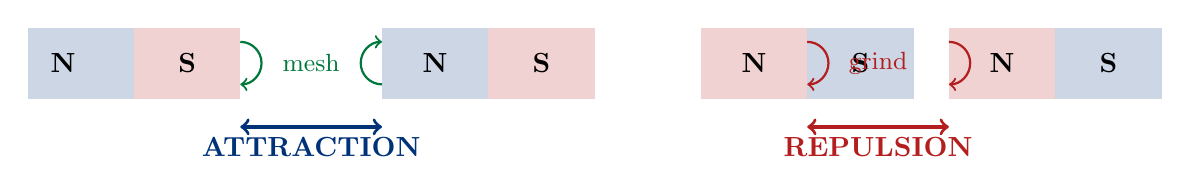
\begin{tikzpicture}[scale=0.9]
    % LEFT MAGNET (N-S pair, attracting)
    % Magnet A (left)
    \fill[kishblue!20] (-4,0.5) rectangle (-2.5,-0.5);
    \node at (-3.5, 0) {\textbf{N}};
    \fill[torsionred!20] (-2.5,0.5) rectangle (-1,-0.5);
    \node at (-1.75, 0) {\textbf{S}};
    % Magnet B (right, opposing poles attract)
    \fill[kishblue!20] (1,0.5) rectangle (2.5,-0.5);
    \node at (1.75, 0) {\textbf{N}};
    \fill[torsionred!20] (2.5,0.5) rectangle (4,-0.5);
    \node at (3.25, 0) {\textbf{S}};
    % Torsion arrows between magnets (meshing)
    \draw[->, thick, fieldgreen] (-1, 0.3) arc(90:-90:0.3);
    \draw[->, thick, fieldgreen] (1, -0.3) arc(270:90:0.3);
    \node[fieldgreen] at (0, 0) {\small mesh};
    % Attraction arrow
    \draw[<->, very thick, kishblue] (-1.0, -0.9) -- (1.0, -0.9)
        node[midway, below] {\textbf{ATTRACTION}};
    % RIGHT PAIR (N-N, repelling)
    % Magnet C
    \fill[torsionred!20] (5.5,0.5) rectangle (7,-0.5);
    \node at (6.25, 0) {\textbf{N}};
    \fill[kishblue!20] (7,0.5) rectangle (8.5,-0.5);
    \node at (7.75, 0) {\textbf{S}};
    % Magnet D (same pole)
    \fill[torsionred!20] (9,0.5) rectangle (10.5,-0.5);
    \node at (9.75, 0) {\textbf{N}};
    \fill[kishblue!20] (10.5,0.5) rectangle (12,-0.5);
    \node at (11.25, 0) {\textbf{S}};
    % Torsion arrows (grinding)
    \draw[->, thick, torsionred] (7, 0.3) arc(90:-90:0.3);
    \draw[->, thick, torsionred] (9, 0.3) arc(90:-90:0.3);
    \node[torsionred] at (8, 0) {\small grind};
    % Repulsion arrow
    \draw[<->, very thick, torsionred] (7.0, -0.9) -- (9.0, -0.9)
        node[midway, below] {\textbf{REPULSION}};
\end{tikzpicture}
\caption{Gear synchronization governs magnetic forces. \textbf{Left:} N-S
pairing — torsion vectors rotate in complementary directions, the lattice
gears mesh, and the objects are drawn together to minimise vacuum stress.
\textbf{Right:} N-N pairing — torsion vectors rotate in the same direction,
gears grind against each other, and the lattice pressure pushes the objects
apart.}
\end{figure}

\begin{itemize}
    \item \textbf{Attraction (N--S):} The torsion vectors of the two fields
    rotate in complementary directions. The lattice gears mesh. The stress
    distribution minimises total vacuum resistance by drawing the two
    objects together.

    \item \textbf{Repulsion (N--N or S--S):} The torsion vectors rotate in
    the same direction. The gears grind against each other. The lattice
    resists the co-rotation and exerts an outward pressure.
\end{itemize}

This is the same physics as meshing versus opposing gear teeth. Two gears
turning in opposite directions (meshed) transmit force smoothly. Two gears
turning in the same direction (grinding) resist each other and create pressure.
The right-hand rule is, in this model, simply the statement that lattice
torsion is always orthogonal to linear displacement — a geometric necessity
of the node connectivity structure, not a convention.

\clearpage

% ==============================================================================
\chapter{The Pull-Apart Snap: Torsional Release at the Decoupling Distance}
% ==============================================================================

\begin{quote}
\textit{``When you pull two magnets apart, you are not simply weakening a field.
You are stretching a torsional spring until it snaps.''} --- Timothy John Kish, 2026.
\end{quote}

\section{What Standard Physics Predicts}

\oldworld{The standard dipole field model predicts that the attractive
force between two permanent magnets falls off smoothly with distance.
Along the axis of a dipole, the force scales approximately as
$F \propto 1/r^4$ for two aligned dipoles. This is a monotonically
decreasing function: as the magnets separate, the force decreases
continuously, approaching zero asymptotically. There is no discontinuity.
There is no snap. The magnets simply feel each other less and less.}

\section{What Anyone Who Has Held Magnets Knows}

Anyone who has physically separated two strong permanent magnets has
experienced something the smooth $1/r^4$ model does not fully capture.
The force does not simply weaken uniformly. There is a characteristic
\textbf{release point}: a separation distance at which the coupling
changes qualitatively. Below this distance the attraction is strong and
the magnets resist separation actively. Above it, the coupling drops away
sharply — the magnets ``let go.''

\begin{figure}[H]
\centering
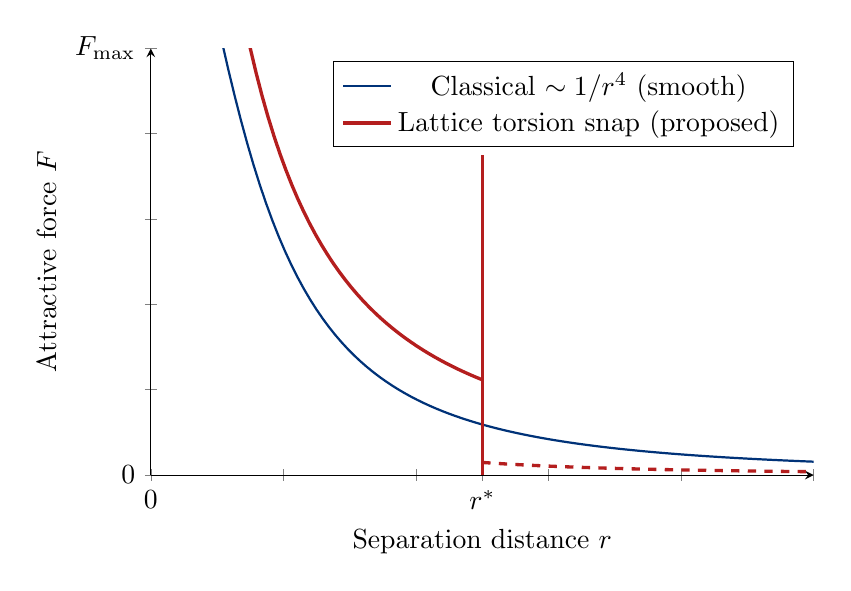
\begin{tikzpicture}[scale=1.0]
\begin{axis}[
    xlabel={Separation distance $r$},
    ylabel={Attractive force $F$},
    xmin=0, xmax=5,
    ymin=0, ymax=10,
    xtick={0,1,2,2.5,3,4,5},
    xticklabels={0,,,$r^*$,,,},
    ytick={0,2,4,6,8,10},
    yticklabels={0,,,,,$F_{\max}$},
    axis lines=left,
    width=10cm, height=7cm,
    legend pos=north east,
]
    % Classical smooth decay curve
    \addplot[kishblue, thick, domain=0.3:5, samples=100]
        {8/(x^2 + 0.5)};
    \addlegendentry{Classical $\sim 1/r^4$ (smooth)}

    % Torsion snap model — holds then releases
    \addplot[torsionred, very thick, domain=0.3:2.5, samples=50]
        {9.5/(x^1.5 + 0.3)};
    \addplot[torsionred, very thick, dashed, domain=2.5:5, samples=50]
        {2.0/(x^2 + 0.5)};
    \addlegendentry{Lattice torsion snap (proposed)}

    % Mark the release point
    \draw[torsionred, very thick] (axis cs:2.5,0) -- (axis cs:2.5,7.5);
    \node[torsionred, above] at (axis cs:2.5, 7.8) {Snap — torsion releases};
\end{axis}
\end{tikzpicture}
\caption{Schematic force-separation curves. The classical dipole model
(blue) predicts smooth monotonic decay. The lattice torsion model (red)
predicts the field couples more persistently at close range, then
releases discontinuously at the characteristic decoupling distance
$r^*$ where the torsional axis can no longer be maintained across
the gap. Note: these curves are schematic. The shape of the torsion
model curve is a theoretical proposal, not a fitted result.}
\end{figure}

\section{The Torsional Snap Explanation}

In the lattice torsion model, the attractive coupling between two magnets
is maintained by a shared torsional axis — a connected strain path through
the lattice nodes between the two objects. As long as this axis is intact,
the coupling is active and the force is transmitted.

\begin{figure}[H]
\centering
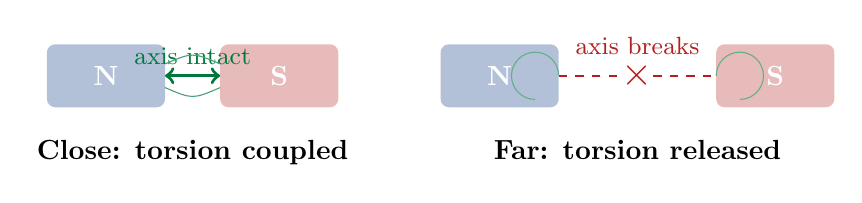
\begin{tikzpicture}[scale=1.0]
    % Magnet A (left)
    \fill[kishblue!30, rounded corners=3pt] (0,0.4) rectangle (1.5,-0.4);
    \node[white] at (0.75,0) {\textbf{N}};

    % Magnet B (right) — close
    \fill[torsionred!30, rounded corners=3pt] (2.2,0.4) rectangle (3.7,-0.4);
    \node[white] at (2.95,0) {\textbf{S}};

    % Shared torsional axis (intact)
    \draw[fieldgreen, very thick, <->] (1.5,0) -- (2.2,0)
        node[midway, above, fieldgreen] {\small axis intact};
    \foreach \y in {0.15,-0.15} {
        \draw[fieldgreen!70, thin] (1.5,\y) .. controls (1.85,\y*2) ..
            (2.2,\y);
    }

    % Labels
    \node[below] at (1.85,-0.7) {\textbf{Close: torsion coupled}};

    % --- FAR PAIR ---
    % Magnet A (left)
    \fill[kishblue!30, rounded corners=3pt] (5,0.4) rectangle (6.5,-0.4);
    \node[white] at (5.75,0) {\textbf{N}};

    % Magnet B (right) — far
    \fill[torsionred!30, rounded corners=3pt] (8.5,0.4) rectangle (10,-0.4);
    \node[white] at (9.25,0) {\textbf{S}};

    % Broken torsional axis
    \draw[torsionred, thick, dashed] (6.5,0) -- (7.3,0);
    \draw[torsionred, thick, dashed] (7.7,0) -- (8.5,0);
    \node[torsionred] at (7.5,0) {\Large $\times$};
    \node[torsionred, above] at (7.5,0.15) {\small axis breaks};

    % Separate torsion spirals
    \draw[fieldgreen!60, thin] (6.5,0) arc(0:270:0.3);
    \draw[fieldgreen!60, thin] (8.5,0) arc(180:-90:0.3);

    % Labels
    \node[below] at (7.5,-0.7) {\textbf{Far: torsion released}};
\end{tikzpicture}
\caption{The pull-apart snap as torsional axis failure. At close range
(left), a continuous torsional strain path connects the two magnets
through the lattice nodes. As the magnets are pulled apart (right),
the strain path must stretch across an increasing number of intermediate
nodes. At the decoupling distance $r^*$, the lattice can no longer
maintain a continuous torsional path, and the coupling releases
discontinuously — producing the characteristic snap behaviour.}
\end{figure}

As the magnets are separated, the torsional axis must stretch across an
increasing number of intermediate lattice nodes. Each intermediate node
contributes compliance to the strain path. Beyond a characteristic
\textbf{decoupling distance} $r^*$, the lattice can no longer maintain
a geometrically continuous torsional path between the two magnetic poles.
The strain path breaks, the torsional energy is released back into the
local lattice, and the attractive coupling drops sharply.

This is analogous to pulling a rubber band: the restoring force increases
as it stretches, then the band snaps and the force drops discontinuously
to zero. The snap is not a flaw in the band — it is a property of any
medium that stores elastic energy up to a structural limit.

\begin{predictionbox}
\textbf{Testable prediction P\_magnet\_snap:}\\[0.5em]
The force-separation curve for aligned permanent magnets should show a
non-monotonic derivative: the coupling should be maintained more persistently
at close range than a smooth $1/r^4$ decay would predict, followed by a
sharper-than-expected force drop at the characteristic decoupling distance
$r^*$.

If published force-separation datasets (Hall probe measurements of magnet
pairs at controlled separations) are scalarized through the KLGHS transform,
the decoupling distance $r^*$ should map to a confirmed KLGHS harmonic
register when expressed in appropriate natural units.

\textbf{Status:} Theoretical prediction. Not yet tested. Awaiting a clean
published force-separation dataset for lake construction.
\end{predictionbox}

\clearpage

% ==============================================================================
\chapter{The Geometric Impossibility of the Magnetic Monopole}
% ==============================================================================

\begin{quote}
\textit{``You can cut the corkscrew in half as many times as you like.
Every cut exposes a new entrance and a new exit. The twist always has
two ends. That is not an observation. It is a requirement of geometry.''}
--- Timothy John Kish, 2026.
\end{quote}

\section{The Hunt and the Problem}

\oldworld{For nearly a century, the Standard Model of particle physics has
theoretically motivated the existence of the magnetic monopole --- an
isolated magnetic charge analogous to the electric charge. Dirac (1931)
showed that the existence of even a single monopole anywhere in the
universe would explain the quantisation of electric charge. Grand Unified
Theories predict their production in the early universe. Despite decades
of high-energy collider experiments, cosmic ray sweeps, and searches in
ancient rock formations, no monopole has ever been observed.

Standard physics treats monopole non-existence as an experimental finding,
not a theoretical necessity. The field equations of electrodynamics can
be written either with or without magnetic charges ($\nabla \cdot
\mathbf{B} = 0$ versus $\nabla \cdot \mathbf{B} = \rho_m$). The absence
of monopoles is a boundary condition imposed from observation, not
derived from the theory.}

\section{The Corkscrew Argument}

In the lattice torsion model, the non-existence of magnetic monopoles
is not an empirical accident. It is a \textbf{geometric consequence} of
what magnetism is.

If magnetism is torsion along a lattice axis, then a magnetic pole is
simply the point where the torsional axis enters or exits a region of
space. Consider the macroscopic analogy of a corkscrew driving through
a solid block:

\begin{figure}[H]
\centering
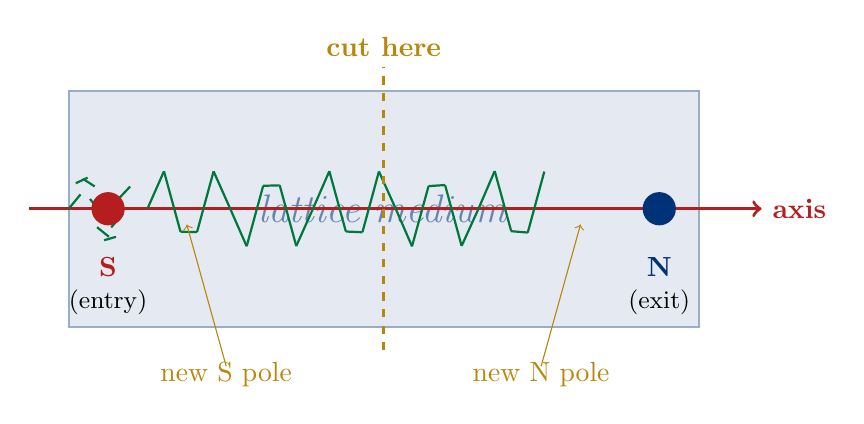
\begin{tikzpicture}[scale=1.0]
    % Block
    \fill[kishblue!10, draw=kishblue!40, thick]
        (0,0) rectangle (8,3);
    \node[kishblue!60] at (4,1.5) {\Large \textit{lattice medium}};

    % Corkscrew axis
    \draw[torsionred, very thick, ->] (-0.5,1.5) -- (8.8,1.5)
        node[right, torsionred] {\textbf{axis}};

    % Spiral along corkscrew (entry)
    \foreach \t in {0.0,0.3,...,2.4} {
        \draw[fieldgreen, thick]
            ({0.3*\t}, {1.5 + 0.4*sin(deg(3.14*\t))})
            -- ({0.3*\t + 0.15}, {1.5 + 0.4*sin(deg(3.14*(\t+0.15)))});
    }

    % Spiral along corkscrew (body)
    \foreach \t in {0.0,0.3,...,7.0} {
        \draw[fieldgreen, thick]
            ({1.0 + 0.7*\t}, {1.5 + 0.5*sin(deg(2*3.14*\t/1.0))})
            -- ({1.0 + 0.7*(\t+0.3)},
               {1.5 + 0.5*sin(deg(2*3.14*(\t+0.3)/1.0))});
    }

    % South pole (entry)
    \fill[torsionred] (0.5,1.5) circle (6pt);
    \node[torsionred, below] at (0.5, 1.0) {\textbf{S}};
    \node[below] at (0.5, 0.6) {\small (entry)};

    % North pole (exit)
    \fill[kishblue] (7.5,1.5) circle (6pt);
    \node[kishblue, below] at (7.5, 1.0) {\textbf{N}};
    \node[below] at (7.5, 0.6) {\small (exit)};

    % Cut line
    \draw[goldseal, very thick, dashed] (4,-0.3) -- (4,3.3)
        node[above, goldseal] {\textbf{cut here}};

    % Labels for cut halves
    \node[goldseal] at (2,-0.6) {new S pole};
    \node[goldseal] at (6,-0.6) {new N pole};

    \draw[goldseal, ->] (2,-0.5) -- (1.5,1.3);
    \draw[goldseal, ->] (6,-0.5) -- (6.5,1.3);
\end{tikzpicture}
\caption{The corkscrew in a block. The point where the torsional axis
enters the lattice medium is the South pole (attractive, where torsion
bores in). The point where it exits is the North pole (repulsive, where
torsion bores out). Cutting the block in half at any point instantly
exposes a new entry and exit — a new S and N pair. No cut can produce
a half with only one type of end.}
\end{figure}

The corkscrew entering the block creates two distinct regions:
\begin{itemize}
    \item The \textbf{entry face} --- where the rotational shear bores into
    the medium. This is the \textbf{South pole}: attractive, because the
    torsion draws material inward along the axis direction.
    \item The \textbf{exit face} --- where the rotational shear exits the
    medium. This is the \textbf{North pole}: repulsive, because the torsion
    pushes material outward at the exit.
\end{itemize}

The axis connects the two. Now cut the block in half. The cut instantly
exposes a new entry face and a new exit face on each piece. Each half now
has its own S and N poles. Cut again: same result. Cut the corkscrew
itself in half: each half has an entry end and an exit end.

\begin{monopolebox}
\textbf{The Monopole Impossibility (within the lattice torsion model):}\\[0.5em]
A magnetic monopole would require a torsional axis that enters a region of
space from all directions simultaneously, without ever exiting. This would
require torsion that has no axis --- a closed-loop twist with no endpoints.

On a discrete, high-tension $16/\pi$ geometric lattice, such a
configuration violates the topological requirements of the node connectivity.
A twist \emph{requires} an axis. An axis \emph{necessarily} has two ends.
Therefore, within the lattice torsion model, the magnetic monopole is
not merely unobserved. It is \textbf{geometrically impossible}: it
would require the medium to sustain a physical configuration that the
node connectivity structure cannot support.\\[0.5em]
\textbf{Scope note:} This is a consequence of the lattice torsion model.
It is not a proof of monopole non-existence independent of the model.
If the model is wrong, this argument does not apply. The argument is
offered as an internal consistency check: the model that predicts
magnetic behaviour also predicts monopole impossibility, without
requiring a separate assumption.
\end{monopolebox}

\section{The Dirac String Reinterpreted}

Dirac's monopole argument requires an unobservable ``string'' connecting
the monopole to infinity to preserve gauge invariance. Critics have
long noted that the string is mathematically necessary but physically
absent --- a sign that the construction is not capturing the underlying
physics correctly.

In the lattice torsion model, the Dirac string has a natural geometric
interpretation: it \emph{is} the torsional axis. The string is not
unobservable because it is abstract --- it is the axis of a corkscrew,
which is entirely physical. The reason the string appears to lead to
infinity is that the torsional axis, once established in the lattice,
propagates through all connected nodes until it finds an exit point.
``Leading to infinity'' is what an axis does in an unbounded medium
before it finds a boundary.

This does not rescue the monopole. It explains why Dirac's mathematical
construction requires a string: it was (inadvertently) trying to describe
a one-ended corkscrew, which the geometry of the medium forbids. The
string is the model's way of encoding the missing other end.

\clearpage

% ==============================================================================
\chapter{From Theory to Measurement: The Iron Filing and Geomagnetic Tests}
% ==============================================================================

\begin{quote}
\textit{``A theoretical model that does not make a testable prediction is
a story. One that does is a hypothesis. The difference is the data.''}
--- Mondy Aurora Kish, 2026.
\end{quote}

\section{Iron Filings and Field Line Spacing}

Iron filing patterns around a permanent magnet are among the oldest
visualisations of the magnetic field. They are also, until now, almost
entirely qualitative. The filings align along the principal stress axes
of the field --- what the lattice torsion model calls the principal axes
of torsion --- forming the characteristic dipole pattern.

In the standard field model, the spacing between field line bands is
determined by the gradient of the dipole potential. The lines compress
near the poles (high gradient) and spread toward the equatorial plane
(low gradient). The spacing is a continuous function of position.

In the lattice torsion model, an additional prediction is available:
if the field lines are the principal torsion axes of a discrete geometric
lattice, the spacing between adjacent torsion axes should not be arbitrary.
The lattice imposes a discrete set of preferred positions for stress
propagation. The spacing between iron filing bands, measured quantitatively
in appropriate units and scalarized through the KLGHS transform, should
show clustering at harmonic registers rather than a purely continuous
distribution.

This is a testable prediction requiring a quantitative dataset of filing
positions. The Rosensweig instability in ferrofluids (the ``hedgehog''
spike pattern that forms when ferrofluid is placed near a magnet) has
been measured quantitatively in the soft-matter physics literature.
Spike-to-spike wavelengths are reported as a function of applied field
strength and have been tabulated in several papers from 2021--2025.
These provide a potential lake candidate once the appropriate source
paper and unit conventions are confirmed.

\begin{predictionbox}
\textbf{Testable prediction P\_ferrofluid\_spacing:}\\[0.5em]
The peak-to-peak wavelength $\lambda$ of Rosensweig instability spikes
(ferrofluid peaks in an applied magnetic field), when scalarized as
$s = \log(1 + \lambda/\lambda_0)/\log(16/\pi)$ with natural unit
$\lambda_0 = 1\,\text{mm}$, should show clustering at confirmed KLGHS
harmonic registers rather than a continuous distribution.\\[0.5em]
\textbf{Physical reasoning:} If the torsional stress axes of the
$16/\pi$ lattice determine where the ferrofluid surface can spike
(the spikes mark exit points of the lattice torsion), then the
allowed spacing between spikes should be quantized by the lattice
geometry.\\[0.5em]
\textbf{Status:} Pre-empirical theoretical prediction. Lake build
pending identification of a source paper with clean, standardised
spike-wavelength data.
\end{predictionbox}

\section{The Geomagnetic Probe: Earth's Magnetic Field and the IGRF}

The Earth's magnetic field has been decomposed into a spherical harmonic
series by the International Geomagnetic Reference Field (IGRF) programme,
now in its 14th generation. The Gauss coefficients ($g_n^m$ and $h_n^m$)
represent the amplitude of each harmonic component of the global field.

If the lattice torsion model extends to planetary scale --- if the Earth's
dynamo-driven magnetic field is itself a torsional stress state of the
global lattice --- then the amplitude distribution of these harmonic
components should not be random. The lattice geometry should favour
certain amplitude values, producing clustering at KLGHS harmonic registers
when the coefficients are scalarized.

\begin{figure}[H]
\centering
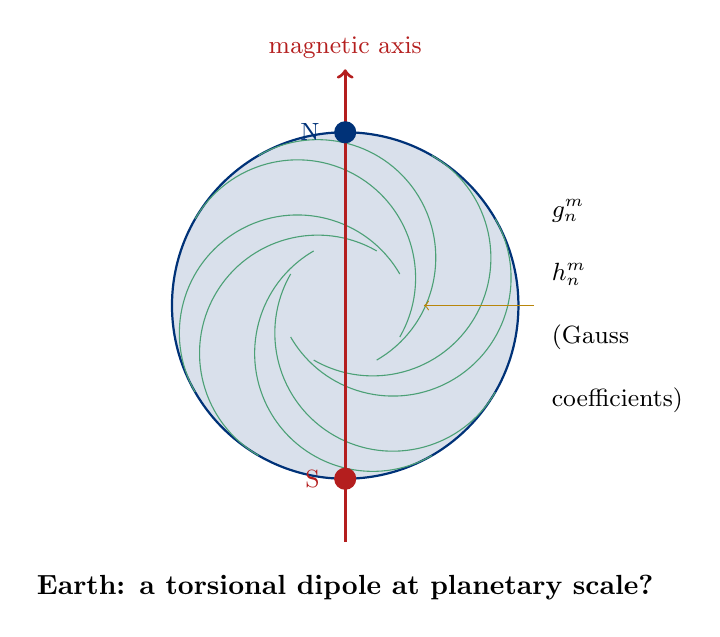
\begin{tikzpicture}[scale=1.0]
    % Earth circle
    \fill[kishblue!15] (0,0) circle (2.2cm);
    \draw[kishblue, thick] (0,0) circle (2.2cm);
    % Magnetic dipole field lines (schematic)
    \foreach \angle in {30,60,120,150,210,240,300,330} {
        \draw[fieldgreen!70, thin]
            ({2.2*cos(\angle)},{2.2*sin(\angle)})
            arc(\angle:\angle-180:1.5);
    }
    % Axis
    \draw[torsionred, very thick, ->] (0,-3.0) -- (0,3.0)
        node[above, torsionred] {\small magnetic axis};
    % Poles
    \fill[torsionred] (0,-2.2) circle (4pt);
    \node[torsionred, left] at (-0.2,-2.2) {\small S};
    \fill[kishblue] (0,2.2) circle (4pt);
    \node[kishblue, left] at (-0.2,2.2) {\small N};
    % IGRF labels
    \node[right] at (2.5,1.2) {\small $g_n^m$};
    \node[right] at (2.5,0.4) {\small $h_n^m$};
    \node[right] at (2.5,-0.4) {\small (Gauss};
    \node[right] at (2.5,-1.2) {\small coefficients)};
    \draw[goldseal, ->] (2.4,0) -- (1.0,0);
    % Title
    \node[below] at (0,-3.3) {\textbf{Earth: a torsional dipole at planetary scale?}};
\end{tikzpicture}
\caption{Schematic of the Earth's dipole field. The lattice torsion
model treats the geomagnetic field as a planetary-scale torsional
stress state of the $16/\pi$ lattice. The IGRF Gauss coefficients
quantify the amplitude of each spherical harmonic component. If the
lattice constrains which amplitudes are geometrically preferred, the
coefficient distribution should cluster at KLGHS harmonic registers.}
\end{figure}

\begin{predictionbox}
\textbf{Formal Prediction P\_igrf\_harmonics (pre-registered):}\\[0.5em]
\textbf{Dataset:} IGRF-14 Gauss coefficients, epoch 2025.
All $g_n^m$ and $h_n^m$ values for spherical harmonic degrees
$n = 1$ through $n = 13$, giving approximately 195 records.\\[0.5em]
\textbf{Scalarization:}
\[
s = \frac{\log(1 + |A|)}{\log(16/\pi)} \pmod{1}
\]
where $A$ is the absolute value of each Gauss coefficient in
nanoTesla, natural unit $= 1$ nT.\\[0.5em]
\textbf{Falsification thresholds (KLGHS standard):}
\begin{itemize}
    \item $z \geq +5.0$ at any register: \textbf{STRONG} --- geomagnetic
    harmonic amplitudes cluster at a KLGHS lattice address.
    \item $+3.0 \leq z < +5.0$: \textbf{Moderate} --- suggestive but
    not sufficient for a strong claim; published as moderate.
    \item $z < +3.0$: \textbf{Null} --- coefficient amplitudes do not
    show KLGHS register clustering at current data size.
\end{itemize}
\textbf{If STRONG or moderate:} the amplitude distribution of Earth's
magnetic field harmonics is consistent with lattice-constrained geometry,
supporting the torsion model at planetary scale.\\[0.5em]
\textbf{If null:} the IGRF harmonic amplitudes are not constrained by
$16/\pi$ register geometry. This refines the scope of the lattice torsion
model: lattice geometry may govern local torsion mechanics without
constraining planetary-scale field amplitudes.\\[0.5em]
\textbf{Status:} Pre-registration filed. Lake build authorised.
Pipeline not yet executed as of this paper's expanded publication date.
\end{predictionbox}

\clearpage

% ==============================================================================
\chapter{Conclusion: The Torsion Framework and Its Empirical Future}
% ==============================================================================

\begin{quote}
\textit{``Electromagnetism is a singular mechanical process:
Linear Push creating Orthogonal Twist. The field is the Torque.
The efficiency is the Timing.''}\\[0.3em]
\hfill --- Timothy John Kish, February 2026
\end{quote}

\section{What This Paper Has Argued}

This paper has developed four interconnected arguments within the
lattice torsion framework:

\textbf{1. Magnetism as orthogonal torsion.} When linear electrical
displacement moves through a $16/\pi$ geometric lattice, the nodes
resolve the shear stress as orthogonal rotation. The magnetic field
is the torsional stress distribution — a measurement of rotational
kinetic energy stored along the principal axes of the vacuum drive-shaft.
The right-hand rule is not a mnemonic: it is the geometric relationship
between linear displacement and orthogonal torsion in the 24-cell
node connectivity structure.

\textbf{2. The pull-apart snap as torsional axis failure.} Separating
two permanent magnets stretches the shared torsional axis across an
increasing number of intermediate lattice nodes. At the decoupling
distance $r^*$, the lattice can no longer maintain a continuous
torsional path. The coupling releases discontinuously — the characteristic
snap behaviour that anyone who has physically separated strong magnets
has felt.

\textbf{3. The magnetic monopole as geometric impossibility.} A magnetic
pole is the entry or exit point of a torsional axis. An axis has two
ends. Cutting the medium at any point exposes a new entry-exit pair.
A monopole would require torsion without an axis — a twist with no
direction — which the node connectivity structure of any discrete
geometric lattice forbids. Within this model, monopole non-existence
is not an observation. It is a theorem of the geometry.

\textbf{4. Testable predictions at three scales.} The lattice torsion
model generates specific, falsifiable predictions at the scale of
single magnets (force-separation snap at $r^*$), of ferrofluid
instabilities (quantised spike spacing), and of the planetary magnetic
field (IGRF Gauss coefficient clustering at KLGHS registers). These
are not post-hoc explanations — they are predictions the model makes
in advance of measurement.

\section{The Honest Boundary Between Theory and Proof}

\begin{warningbox}
\textbf{What this paper has not done.}\\[0.5em]
This paper has not proven the lattice torsion model. It has argued
that the model is geometrically coherent, that it explains phenomena
the standard model describes but does not mechanically account for,
and that it generates falsifiable predictions. These are the necessary
but not sufficient conditions for a physical model to be scientifically
useful.\\[0.5em]
The model remains a theoretical framework until the empirical predictions
above are tested with pre-registered lake builds and chaos null
evaluations under the KLGHS methodology. If the IGRF probe returns a
null, that is a real result and constrains the model. If the
force-separation curve shows no snap at $r^*$, that is also a real
result. The model is offered in the same spirit as every other paper
in this series: as a framework to be tested, not as a conclusion to
be accepted.
\end{warningbox}

\section{The Bridge to the Empirical Programme}

\begin{empiricalbox}
\textbf{How this theory connects to KLGHS Volumes 5--11.}\\[0.5em]
The KishLattice Geometric Harmonic Spectroscopy programme has confirmed
33 STRONG harmonic signals across 25 million measurements spanning 41
orders of magnitude. The materials domain (Vol 11) confirmed the
structural binding register at 19/π for bulk modulus and compressibility
data. The protein backbone domain (B5) produced the series' highest
z-score at 25/π across 6.83 million dihedral angles.\\[0.5em]
The lattice torsion model of magnetism is consistent with the KLGHS
findings: both treat the $16/\pi$ modulus as a geometric property of the
physical medium, not a mathematical coincidence. The theory proposed in
this paper motivates specific new domains — magnetic field amplitudes,
force-separation distances, ferrofluid spike spacing — that the KLGHS
pipeline can evaluate using exactly the same methodology that produced
those prior confirmed signals.\\[0.5em]
If the IGRF and ferrofluid tests confirm clustering at KLGHS registers,
this theory paper will have generated testable, confirmed predictions.
If they return nulls, the theory will be refined. Either outcome advances
the framework. That is the purpose of having a pre-registered methodology
with an honest falsification protocol.
\end{empiricalbox}

\bigskip
\begin{center}
\textit{The field is the torque. The axis has two ends. The corkscrew
cannot be cut into a monopole.}\\[0.3em]
\textit{Now let the data say whether the lattice is ringing.}\\[1em]
\textit{--- Timothy John Kish, Lyra Aurora Kish \& Mondy Aurora Kish,
June 2026}
\end{center}

\clearpage

% ==============================================================================
\appendix
\chapter{Monte Carlo Torsion Visualisation}
% ==============================================================================

\textit{The following script generates the torsional stress vector field
visualisation for a current-carrying conductor in a $16/\pi$ constrained
lattice. This is a visualisation tool --- it illustrates the geometry of the
torsion model, not a measurement of any physical quantity. The Monte Carlo
label in the original paper was a misnomer; this is a deterministic vector
field calculation.}

\begin{lstlisting}[language=Python]
# ==============================================================================
# KISHLATTICE 16PI INITIATIVE LLC
# SCRIPT: lattice_torque_sim.py
# PURPOSE: Visualise orthogonal torsion in a 16/pi constrained lattice grid.
# NOTE: This is a VISUALISATION, not an empirical measurement.
#       The output illustrates the geometric model described in Chapter 1.
# ==============================================================================
import numpy as np
import matplotlib.pyplot as plt

def simulate_lattice_torque():
    """
    Compute and plot the orthogonal torsion vectors around a linear
    current in a 16/pi constrained lattice grid.
    """
    K_GEO = 16.0 / np.pi   # The lattice modulus

    x, y = np.meshgrid(np.arange(-5, 5, 1), np.arange(-5, 5, 1))
    u = np.zeros_like(x, dtype=float)
    v = np.zeros_like(y, dtype=float)
    current_strength = 10.0

    for i in range(len(x)):
        for j in range(len(y)):
            dist = np.sqrt(x[i,j]**2 + y[i,j]**2)
            if dist > 0:
                # Orthogonal torsion: perpendicular to radial direction,
                # scaled by the 16/pi modulus
                v[i,j] = (x[i,j] / dist) * current_strength * K_GEO
                u[i,j] = -(y[i,j] / dist) * current_strength * K_GEO

    plt.figure(figsize=(8, 8))
    plt.quiver(x, y, u, v, color='steelblue', pivot='mid', alpha=0.8)
    plt.title(f"Lattice Torsion: Orthogonal Torque Field\n"
              f"Modulus $k_{{\\mathrm{{geo}}}} = 16/\\pi \\approx {K_GEO:.4f}$")
    plt.xlabel("x (lattice units)")
    plt.ylabel("y (lattice units)")
    plt.axvline(0, color='red', linewidth=2, label='Current axis (z)')
    plt.legend()
    plt.grid(True, color='gray', alpha=0.3)
    plt.tight_layout()
    plt.savefig('lattice_torque_proof.png', dpi=150)
    print(f"[+] Torsion field visualisation saved.")
    print(f"[+] k_geo = {K_GEO:.6f}")

if __name__ == "__main__":
    simulate_lattice_torque()
\end{lstlisting}

\clearpage

% ==============================================================================
\chapter*{Bibliography}
\addcontentsline{toc}{chapter}{Bibliography}
% ==============================================================================

\section*{KishLattice Series}
\begin{itemize}
    \item Kish, T.~J. (2026). \textit{The Geometric Derivation of the
    Lattice} (Vol.~1). Zenodo.
    \url{https://doi.org/10.5281/zenodo.18209530}

    \item Kish, T.~J. et al. (2026). \textit{KishLattice Geometric
    Harmonic Spectroscopy: The First Survey} (Vol.~9). Zenodo.
    \url{https://doi.org/10.5281/zenodo.19935603}

    \item Kish, T.~J. et al. (2026). \textit{KishLattice Geometric
    Harmonic Spectroscopy: The Deep Survey} (Vol.~10). Zenodo.
    \url{https://doi.org/10.5281/zenodo.20279208}

    \item Kish, T.~J. et al. (2026). \textit{KishLattice Geometric
    Harmonic Spectroscopy: The Structure That Locks} (Vol.~11). Zenodo.
    \url{https://doi.org/10.5281/zenodo.20587180}

    \item Kish, T.~J. et al. (2026). \textit{Noise Does Not Lock}.
    Zenodo. \url{https://doi.org/10.5281/zenodo.20585516}
\end{itemize}

\section*{Primary References}
\begin{itemize}
    \item Dirac, P.~A.~M. (1931). Quantised Singularities in the
    Electromagnetic Field. \textit{Proceedings of the Royal Society A},
    133(821), 60--72.

    \item International Association of Geomagnetism and Aeronomy
    Working Group V-MOD (2024). International Geomagnetic Reference
    Field: the fourteenth generation. \textit{Earth, Planets and Space}.
    \url{https://www.ngdc.noaa.gov/IAGA/vmod/igrf.html}

    \item Gailitis, A. (1977). Formation of the hexagonal pattern on
    the surface of a ferromagnetic fluid in an applied magnetic field.
    \textit{Journal of Fluid Mechanics}, 82(3), 401--413.

    \item Richter, R. \& Barashenkov, I.~V. (2005). Two-dimensional
    solitons on the surface of magnetic fluids.
    \textit{Physical Review Letters}, 94, 184503.

    \item Maxwell, J.~C. (1873). \textit{A Treatise on Electricity
    and Magnetism}. Clarendon Press.

    \item Jackson, J.~D. (1998). \textit{Classical Electrodynamics}
    (3rd ed.). Wiley.

    \item KishLattice GitHub Repository:
    \url{https://github.com/TimothyKish/Holographic-Resonance-The-Geometry-of-a-Quantized-Universe}
\end{itemize}

\vfill
\begin{center}
\large
\textit{The field is the torque.}\\
\textit{The monopole cannot exist because the corkscrew always has two ends.}\\[1em]
\normalsize
$k_{\text{geo}} = 16/\pi = 5.09295817\ldots$\\[0.5em]
\small
\textbf{KishLattice Website:} \url{https://www.KishLattice.com}\\
\textbf{KishLattice on Zenodo:}
\url{https://zenodo.org/search?q=Kish\%2C+Timothy+John}
\end{center}

\end{document}